\documentclass[a4paper,11pt]{article} % or {article}

\usepackage[utf8x]{inputenc} % utf8x es un extensión, en gral las
% extensiones funcionan mejor, "archx" son extensiones. En ubuntu
% la extensión es utf8x 
\usepackage[spanish]{babel}
\usepackage[T1]{fontenc} % Los fonts tipo T1 están en todos los
% visualizadores
\usepackage{times} % recordar que T1 + times logra un estilo de fuente
%muy armónico
\usepackage{verbatim} % verbatim package to use multiline comments in
%Latex \begin{comment}...\end{comment}

% SOME Extra packages
\usepackage{calc}
\usepackage{setspace}
\usepackage{fixltx2e}
\usepackage{graphicx}
\usepackage{multicol}
\usepackage[normalem]{ulem}
%% Please revise the following command, if your babel
%% package does not support English (US)
\usepackage{color}
\usepackage{hyperref}

%opening
\title{\Large Trabajo Práctico Nº2\\\Large
Televisi\'on y Procesamiento de Im\'agenes (TVPI) \\[2cm]\huge
Dimensionamiento de una estaci\'on ISDB-Tb \& Visita LV80 TV Canal
10 \\[2cm]}
\author{\emph{Barrirero, Exequiel - Gismondi, Gonzalo - Petit,
Victoria y Villagra, Mat\'ias}}
\date{\textit{24/11/11}}


\begin{document}
\pagenumbering{roman}
\maketitle
\thispagestyle{empty}

\begin{figure}[htb] % h= here t=top =bottom con respecto al texto
\centering

\includegraphics[width=.5\textwidth,
keepaspectratio]{/home/delivery/Desktop/TVPILatex/Figuras/LogoUBP.jpg}
%\caption{\emph{ Representaci\'{o}n gr\'{a}fica

\end{figure}
\begin{center}
%\\[6cm]%%%%%%%%%%%%%%%%%%%%%%%%%%%%%%%%%%%%%%%%%%%%%%%%%%%%%%%%%%%%%%%%
\small under \LaTeX
\end{center}

\newpage
\begin{center}
\tableofcontents
\listoffigures
%\listoftables
\end{center}

\newpage
\pagenumbering{arabic}
\setcounter{page}{1}
\section{Dimensionamiento de una estaci\'on ISDB-Tb}

\subsection{Requerimientos de Dise\~no}
La transmisión de Canal 10 noticias (CBA24N) se realiza en la actualidad
emitiendo en canal 31, en norma ISDB-Tb, desde las instalaciones del
Cerro Mogotes, próximo a la Ciudad de Carlos Paz, incluido en la
Plataforma Nacional de TV Digital, desarrollada por el estado nacional.
Actualmente se emite una señal digital SD (31-1), comprimida a 6Mbps, en
Capa A, 13 segmentos, 16-QAM y 1/2, Modo 1 con Intervalo de Guarda 1/4.
La transmisión se origina en forma analógica en las instalaciones de
Canal 10 TV de Córdoba, en el Barrio Marques de Sobremonte, contando con
un enlace analógico que transporta la señal desde el punto de generación
hasta la planta transmisora. 
\\

Se desea pasar a un sistema
demultiprogramación, incorporando en el mismo canal 31 una señal Full HD
(31-2), más otra señal SD (31-3), un One-Seg de la señal HD (31-4) y
datos de interactividad por 0,5 Mbps de bitrate (la interactividad
corresponde a la señal 31-3.


%\subsubsection*{Factores de performance} % el * entre el
%comando y los datos hace que no se nuemere esta sección.

\newpage
\subsection{Modificaciones, incorporaci\'on de dispositivos y
programación del modulador para multiprogramación}

Partiendo de las modificaciones de dise\~no deseadas para el Ch31:

\begin{itemize}
\item 1 Se\~nal Full HD (31-2)
\item 2 Se\~nal SD (31-1 // 31-3) 
\item 1 Se\~nal LD (One-Seg 31-4 from HD) 
\item 1 Flujo de Datos interactivos (close caption, encuestas, etc)
\end{itemize} 

Se sugieren modificaciones en base a los criterios estudiados y
analizados en las clases de TVPI. Como tambi\'en teniendo en cuanta la
implementaci\'on, que se encuentra actualmente funcionando en Canal 10
de la ciudad de C\'ordoba. La cual utiliza encoders tanto en su planta
productora, como en su planta Tx en el cerro Mogote. Esto se
debe a que el radio enlace utilizado de momento es anal\'ogico.
Por lo tanto la se\~nal debe ser redigitalizada (transcodificada)
para su posterior transmisi\'on. Solo a modo complementario, en un
futuro pr\'oximo se planea reemplazar la Tx por radiofrecuencias por un
enlace de fibra \'optica seg\'un comentarios del personal t\'ecnico
durante la visita.
En primer lugar podemos decir que claramente es inviable no utilizar los
\textbf{Encoders} en las instalaciones de Canal 10 TV (B:
Marqu\'es de Sobremonte) para el nuevo sistema de multiprogramación
propuesto. Ya que los BW est\'andares a la entrada del
\textbf{Multiplexor} ser\'an considerables, presentados a
continuaci\'on: 

%\begin{tabular}[htb]{|l|c|}

\begin{itemize}
\item 1 Full HD \ (13 Mbps)
\item 2 SD \ \ \ \ \ \ \ \ \  ( 2 x 3Mbps) 
\item 1 OSeg \ \ \ \ \  ( 0,384 Kbps = 0,4 Mbps)
\item 1 Datos \ \ \ \ \ (0,5 Mbps)
\end{itemize}

Resultando: \textbf{HD + SD + SD (CBA24N) + OS + Datos = 19,9 Mbps}

\begin{figure}[h!] 
\centering
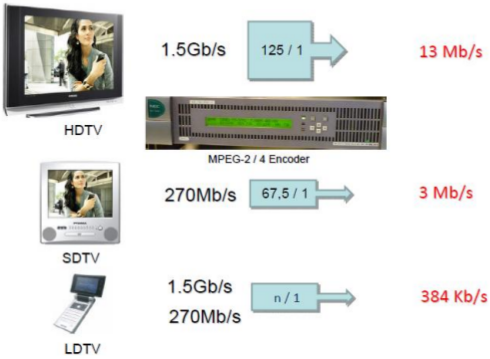
\includegraphics[width=.90\textwidth,
keepaspectratio]{/home/delivery/Desktop/TVPILatex/Figuras/Fig1.png}
\caption{\emph{Diagrama de Digitalizaci\'on y Compresi\'on de un Canal
de TV.}}
\end{figure} 

\begin{figure}[h!] 
\centering
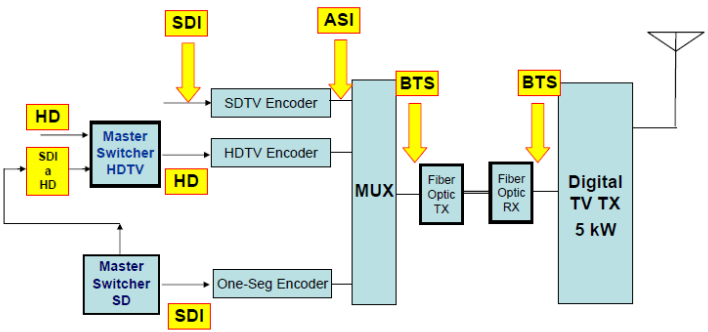
\includegraphics[width=1\textwidth,
keepaspectratio]{/home/delivery/Desktop/TVPILatex/Figuras/Fig3.png}
\caption{\emph{Diagrama en bloques Sistema ISDB-Tb Canal7 Argentina.}}
\end{figure}

\newpage
De esta forma ser\'a posible transmitir se\~nales digitalizadas en
MPEG-2 (TS). Lo que implica un gran ahorro de capacidad en el
radioenlace a la planta Tx, donde ingresaran al
\textbf{Re-Multiplexor}. Aunque corresponde a otra configuraci\'on
topol\'ogica, ser\'ia equivalente al bloque ``MUX'' de la
\textbf{\emph{Figura 2}}. Las incorporaciones y detalles de
tecnolog\'ia de los dispositivos a implementar se presentan en la
\textbf{\emph{Subsecci\'on 1.3.1}}. 

\newpage
Debajo se exponen los resultados obtenidos mediante la
utilizaci\'on de la Calculadora ISDB-Tb, en relaci\'on a la
\textbf{programaci\'on del modulador} para un \textbf{Modo 2}. Los
resultados en respuesta a los par\'ametros seleccionados se analizar\'an
en profundidad en la Secci\'on \textbf{\emph{1.4 Configuración de los
parámetros ISDB-Tb (Modo - TG )}} 

\begin{figure}[h!] 
\centering
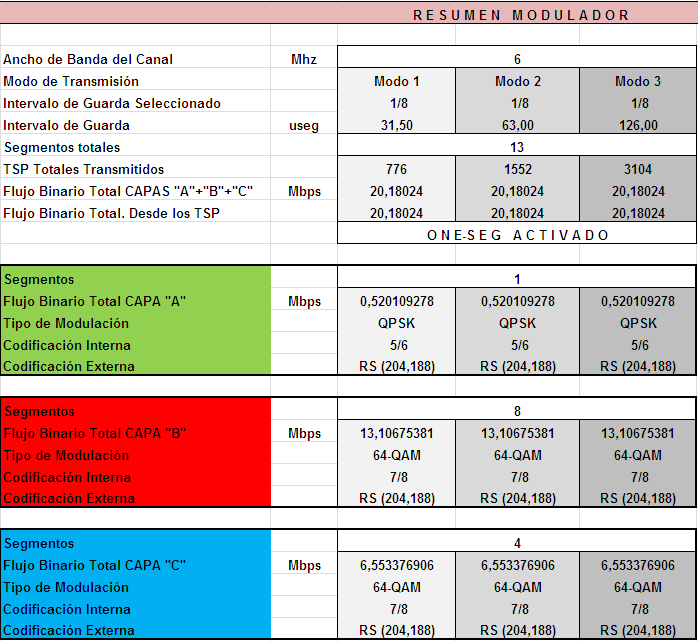
\includegraphics[width=1\textwidth,
keepaspectratio]{/home/delivery/Desktop/TVPILatex/Figuras/Fig4.png}
\caption{\emph{Resumen Modulador Calculadora ISDB-Tb (1er Parte).}}
\end{figure}

\begin{figure}[h!] 
\centering
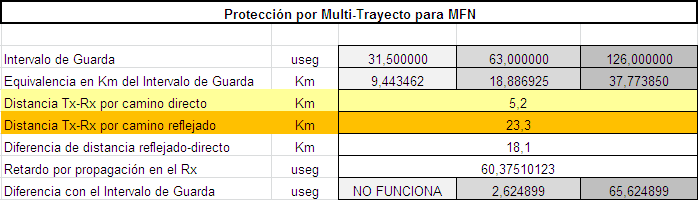
\includegraphics[width=1 \textwidth,
keepaspectratio]{/home/delivery/Desktop/TVPILatex/Figuras/Fig5.png}
\caption{\emph{Resumen Modulador Calculadora ISDB-Tb (2da Parte).}}
\end{figure}  

  
%\end{tabular}

\newpage
\subsection{Diagrama en bloques del sistema desde el switcher de
generación de las señales hasta el modulador}

\begin{figure}[htb] 
\centering
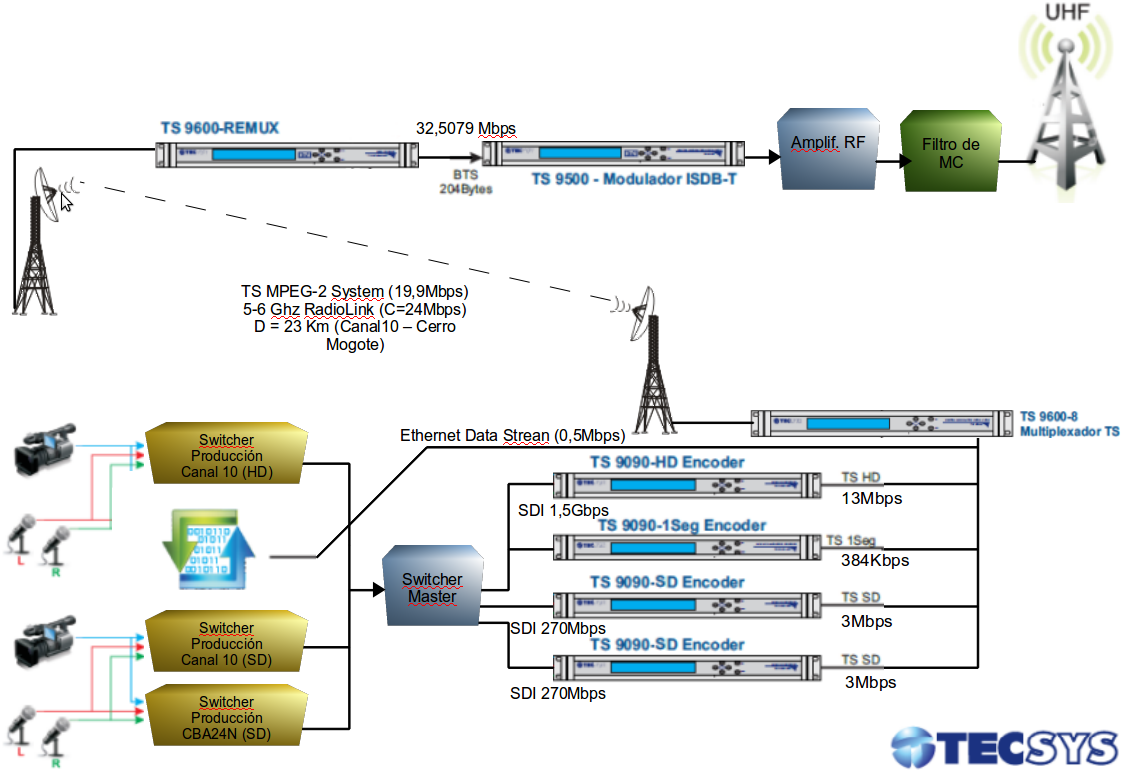
\includegraphics[width=1.1 \textwidth,
keepaspectratio]{/home/delivery/Desktop/TVPILatex/Figuras/Fig6.png}
\caption{\emph{Diagrama en Bloques del Sistema ISDB-Tb
propuesto. Desde el Switcher de generaci\'on de las se\~nales hasta el
modulador. Se presenta a TECSYS solo a modo de ejemplo.}}
\end{figure} 

\newpage
\subsubsection{Tecnolog\'ias necesarias}

Se presentan debajo los posibles equipos para implemenntar la
multiprogramación propuesta:

\begin{itemize}
\item Switcher Master SD/HD (2 Opciones NEC o Utah Scientific). 
\item Encoders MPEG-4 (Z3 MVE-02 / MVE-20). Recordar el traslado del
encoder SD previamente ubicado en planta Tx Cerro Mogote. 
\item TS Multiplexor (2 Opciones AMT DTA-3050 o ERICSSON MX8400).
\item ISDB-Tb Re-multiplexer (NDS3105A - Si bien no se utiliza en la
implementaci\'on propuesta, se recurrir\'a al mismo en secciones
posteriores \textbf{\emph{Subsecci\'on 1.5)}}. 
\end{itemize} 

\begin{figure}[h!] 
\centering
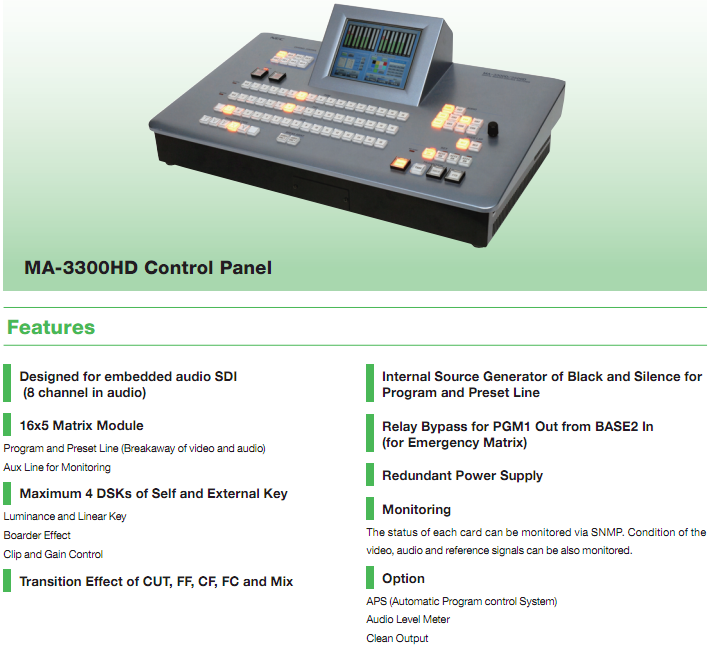
\includegraphics[width=1 \textwidth,
keepaspectratio]{/home/delivery/Desktop/TVPILatex/Figuras/Fig7.png}
\caption{\emph{NEC Corporation MA-3300HD HDTV Digital Master Switcher.
}}
\end{figure} 

\begin{figure}[h!] 
\centering
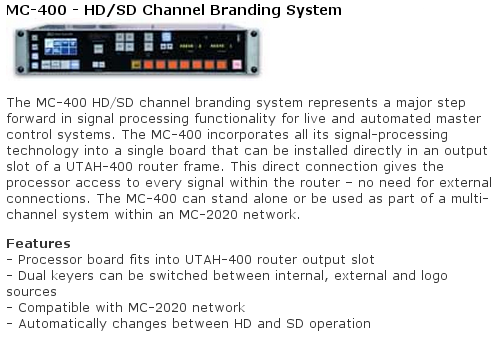
\includegraphics[width=.8 \textwidth,
keepaspectratio]{/home/delivery/Desktop/TVPILatex/Figuras/Fig8.png}
\caption{\emph{Caracter\'isticas Utah Scientific Master
Switcher-400-HD/SD Channel Branding System.
}}
\end{figure} 

%\newpage
%.
\begin{figure}[h!] 
\centering
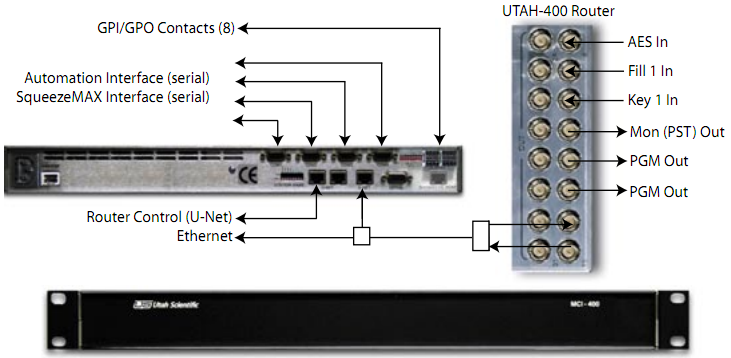
\includegraphics[width=1 \textwidth,
keepaspectratio]{/home/delivery/Desktop/TVPILatex/Figuras/Fig9.png}
\caption{\emph{Interfaces Utah Scientific Master
Switcher-400-HD/SD Channel Branding System.}}
\end{figure}

\begin{figure}[h!] 
\centering
\includegraphics[width=1 \textwidth,
keepaspectratio]{/home/delivery/Desktop/TVPILatex/Figuras/Fig10.png}
\caption{\emph{Z3 MVE-02 / MVE-20 - ISDB-T Broadcast HD, SD and 1-seg
Encoders/Decoders.}}
\end{figure}

\newpage
\begin{figure}[h!] 
\centering
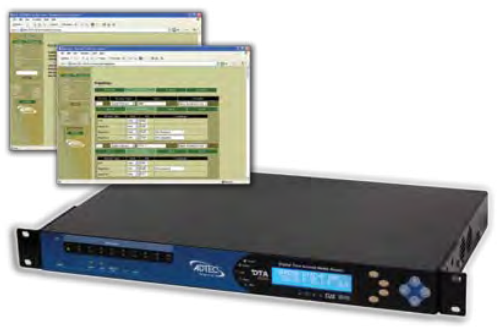
\includegraphics[width=.8 \textwidth,
keepaspectratio]{/home/delivery/Desktop/TVPILatex/Figuras/Fig11.png}
\caption{\emph{Caracter\'isticas AMT DTA-3050 MPEG-2/MPEG-4 TS Router
ASI Multiplexer.}}
\end{figure}

\begin{figure}[h!] 
\centering
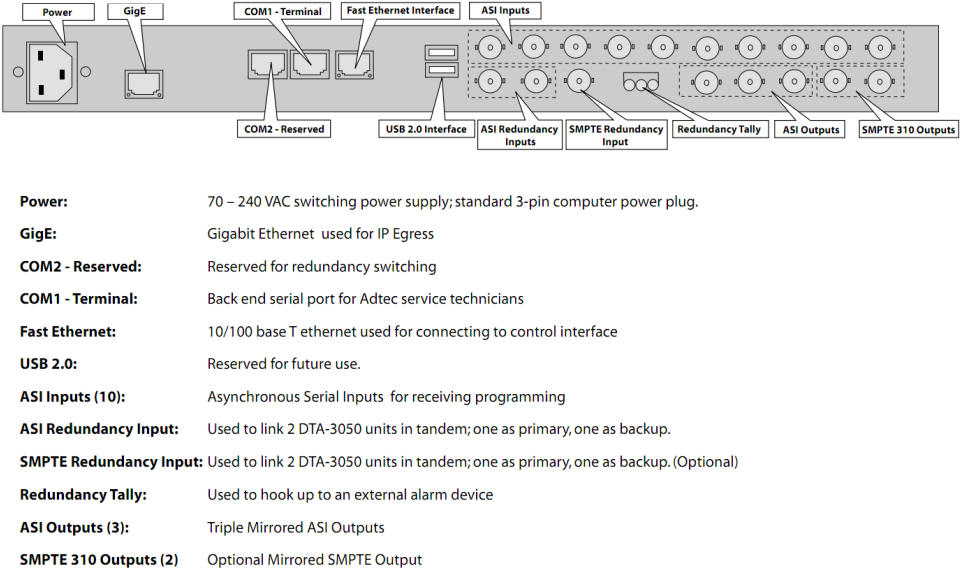
\includegraphics[width=1.1 \textwidth,
keepaspectratio]{/home/delivery/Desktop/TVPILatex/Figuras/Fig12.png}
\caption{\emph{Interfaces AMT DTA-3050 MPEG-2/MPEG-4 TS Router ASI
Multiplexer.}}
\end{figure}

\begin{figure}[h!] 
\centering
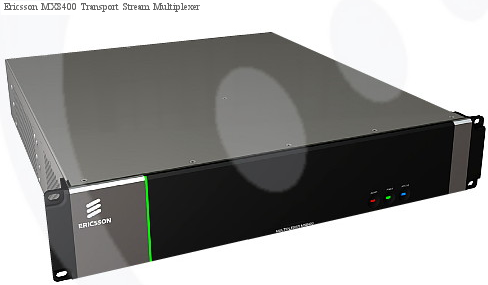
\includegraphics[width=.7 \textwidth,
keepaspectratio]{/home/delivery/Desktop/TVPILatex/Figuras/Fig13.png}
\caption{\emph{ERICSSON MX8400 Transport Stream (TS) Multiplexer.}}
\end{figure}

\begin{figure}[h!] 
\centering
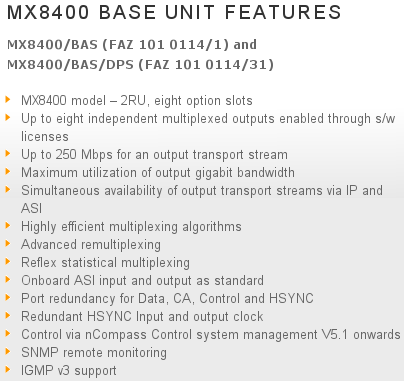
\includegraphics[width=.7 \textwidth,
keepaspectratio]{/home/delivery/Desktop/TVPILatex/Figuras/Fig14.png}
\caption{\emph{Caracter\'isticas ERICSSON MX8400 Transport Stream (TS)
Multiplexer.}}
\end{figure}

\begin{figure}[h!] 
\centering
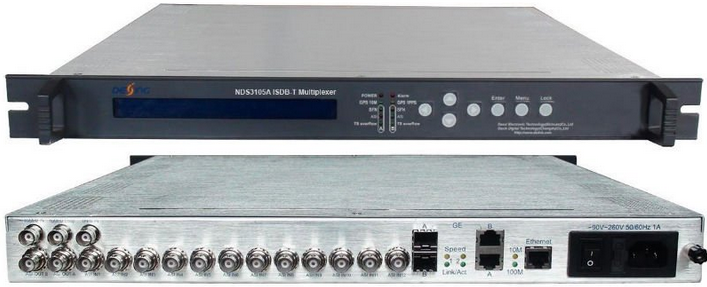
\includegraphics[width=.7 \textwidth,
keepaspectratio]{/home/delivery/Desktop/TVPILatex/Figuras/Fig15.png}
\caption{\emph{NDS3105A ISDB-T Re-Multiplexer.}}
\end{figure}

\begin{figure}[h!] 
\centering
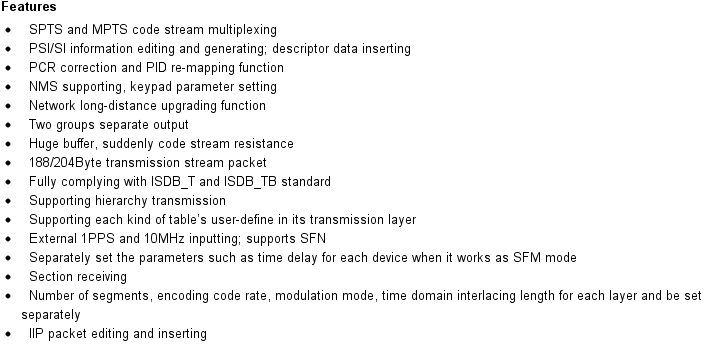
\includegraphics[width=1.1 \textwidth,
keepaspectratio]{/home/delivery/Desktop/TVPILatex/Figuras/Fig16.png}
\caption{\emph{Caracter\'isticas NDS3105A ISDB-T Re-Multiplexer.}}
\end{figure}

\begin{figure}[h!] 
\centering
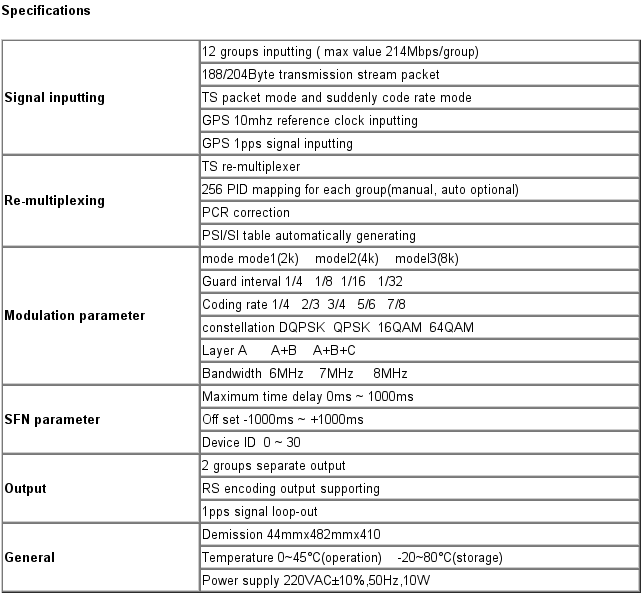
\includegraphics[width=1 \textwidth,
keepaspectratio]{/home/delivery/Desktop/TVPILatex/Figuras/Fig17.png}
\caption{\emph{Especificaciones NDS3105A ISDB-T Re-Multiplexer.}}
\end{figure}

\newpage
\begin{center}
\color{white}{.}
\end{center}
\newpage
\begin{center}
\color{white}{.}
\end{center}
\newpage
\begin{center}
\color{white}{.}
\end{center}
\newpage
\begin{center}
\color{white}{.}
\end{center}
\newpage
\begin{center}
\color{white}{.}
\end{center}
\newpage
\begin{center}
\color{white}{.}
\end{center}
\newpage

\subsubsection{Enlaces necesarios Estudio - Planta Transmisora
Digital}

Se aprecia que las distancia aproximada calculada mediante la
herramiento Google Earth otorga un resultado de 23km. Como se
planteo anteriormente \\ \textbf{R > 19,9 Mbps} por lo tanto se proponen
las siguientes tecnolog\'ias de \\ MOTOROLA => \
\textbf{\emph{21Mbps(PTP-200) \ < \ R \ < \ 25Mbps(PTP-300)}}: 

\begin{figure}[h!] 
\centering
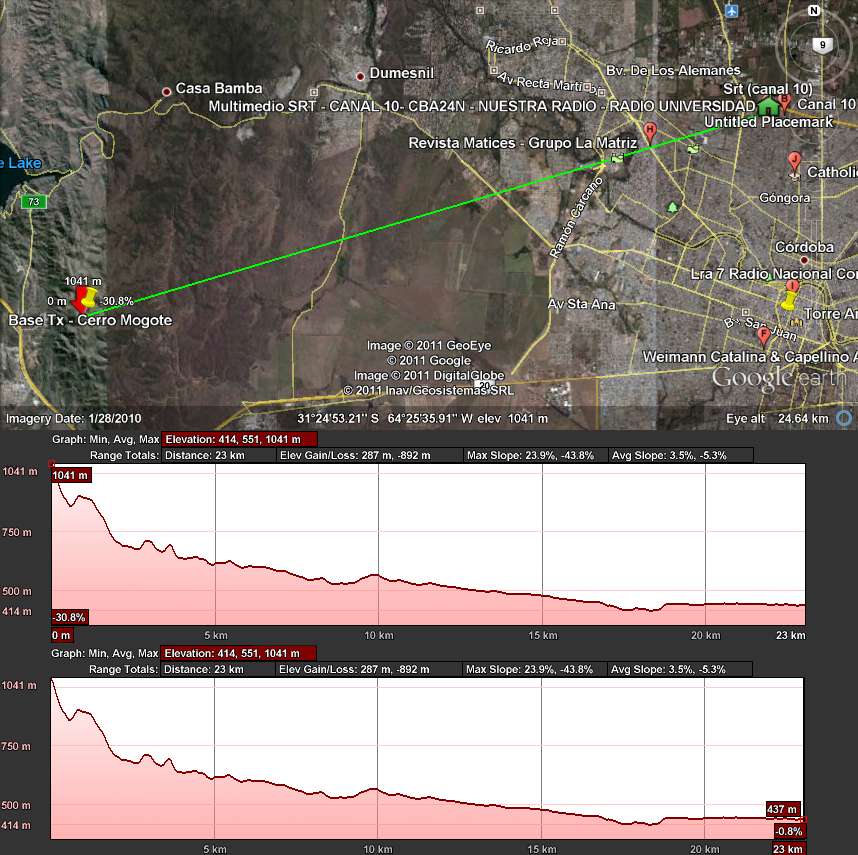
\includegraphics[width=1.2 \textwidth,
keepaspectratio]{/home/delivery/Desktop/TVPILatex/Figuras/Fig22.png}
\caption{\emph{Enlace Digital Point to Point instalaciones Canal 10
(M. de Mojica 1600, 5008 Cba.) a Base Tx Cerro Mogote}}
\end{figure}

\begin{figure}[h!] 
\centering
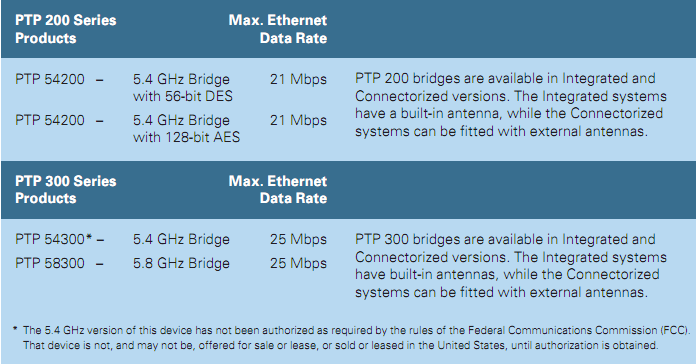
\includegraphics[width=1 \textwidth,
keepaspectratio]{/home/delivery/Desktop/TVPILatex/Figuras/Fig19.png}
\caption{\emph{Motorola Fixed Point-to-Point Wireless Bridge - PTP 200
\& 300 Series Products.}}
\end{figure}

\begin{figure}[h!] 
\centering
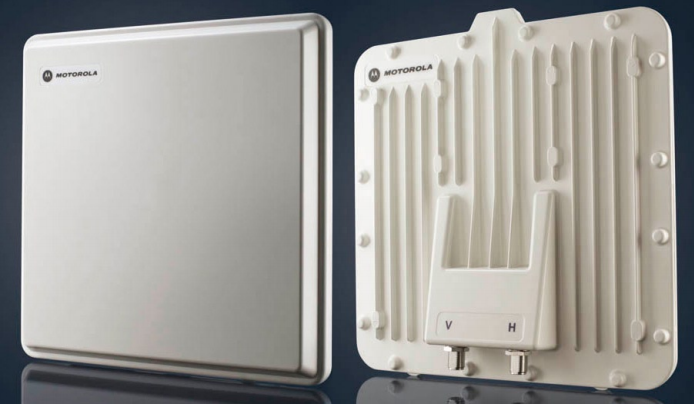
\includegraphics[width=1 \textwidth,
keepaspectratio]{/home/delivery/Desktop/TVPILatex/Figuras/Fig20.png}
\caption{\emph{PTP 200 \& 300 Series Radio.}}
\end{figure}

\begin{figure}[h!] 
\centering
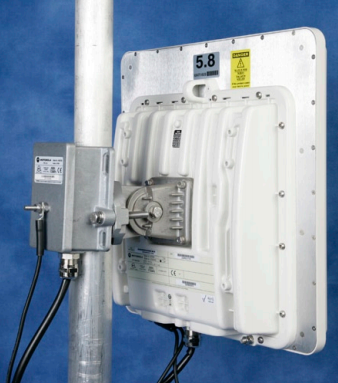
\includegraphics[width=.8 \textwidth,
keepaspectratio]{/home/delivery/Desktop/TVPILatex/Figuras/Fig21.png}
\caption{\emph{Instalated PTP 200 \& 300 Series Radio.}}
\end{figure}

\begin{center}
\color{white}{.}
\end{center}
\newpage
\begin{center}
\color{white}{.}
\end{center}
\newpage
\begin{center}
\color{white}{.}
\end{center}
\newpage

\subsection{Configuraci\'on de los par\'ametros ISDB-Tb (Modo -
T\textsubscript{G}) \& Programaci\'on del Modulador}

\begin{figure}[h!] 
\centering
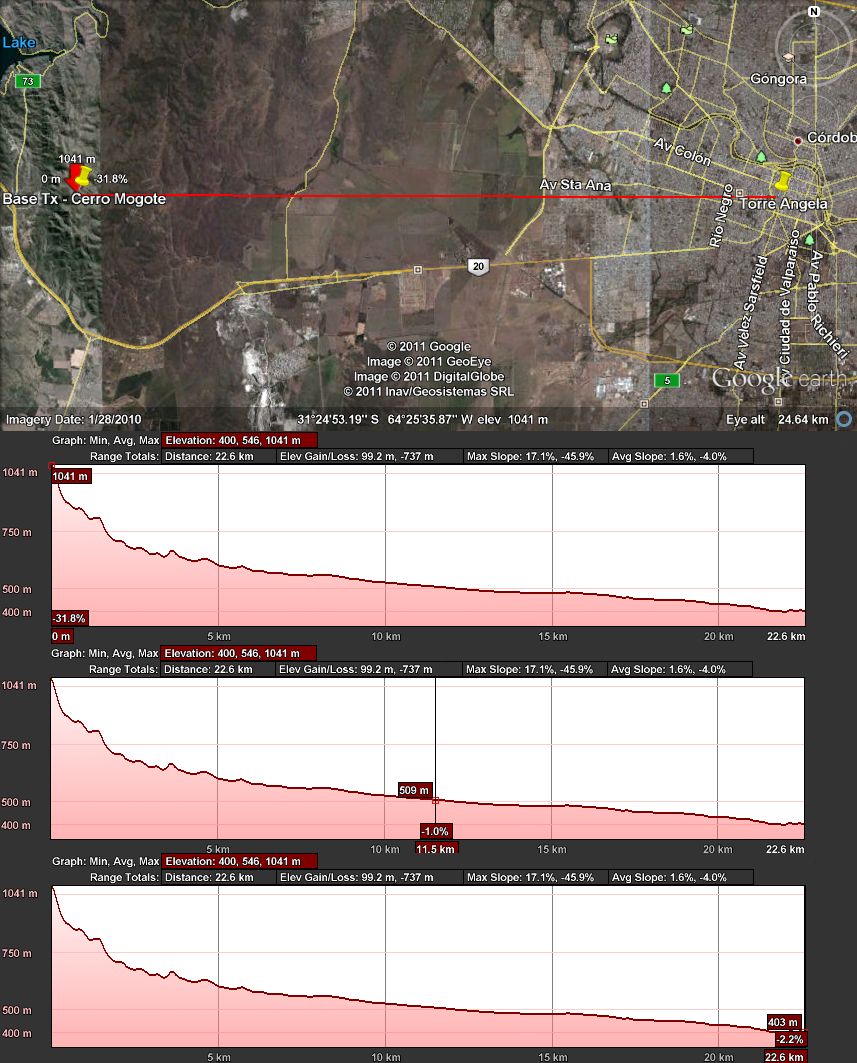
\includegraphics[width=1.10 \textwidth,
keepaspectratio]{/home/delivery/Desktop/TVPILatex/Figuras/Fig18.png}
\caption{\emph{Tx Cerro Mogote al punto de refexi\'on de mayor altura
de la ciudad de Cordoba (Torre Angela), con perfil topogr\'afico.}}
\end{figure}

\begin{figure}[h!] 
\centering
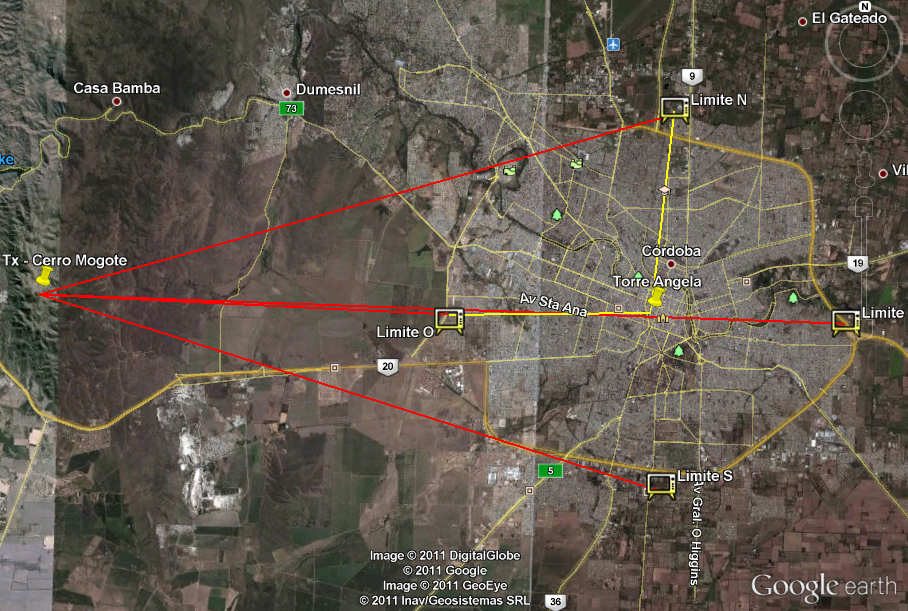
\includegraphics[width=1.10 \textwidth,
keepaspectratio]{/home/delivery/Desktop/TVPILatex/Figuras/Fig30.png}
\caption{\emph{Tx Cerro Mogote a los puntos de cobertura l\'imite N,S,E
y O (Rayos directos en Rojo). Rayos reflejados torre Angela
(amarillo).}}
\end{figure}

Para la configuraci\'on de los par\'ametros ISDB-Tb (Modo y TG). Como
tambi\'en para la configuraci\'on de los par\'ametros del modulador (
C/N, Esquema de modulaci\'on, FEC). Partimos del an\'alisis realizado
del area de cobertura \textbf{\emph{(radio de cobertura libre de ISI
$\Longleftrightarrow$ T\textsubscript{G})}} deseado. Resultando un radio
de aproximadamente 9-10 Km con respecto al centro de la ciudad de
C\'ordoba. M\'as precisamente del punto (estructura) de mayor altura que
inevitablemente producira reflexiones.
Claramente el peor caso se encuentra en el Limite Oeste de
cobertura. Ya que el \\ \\ \textbf{Rayo directo \ \ \ = 14,5 Km} \\
\textbf{Rayo reflejado = 22,6 Km + 10 Km (Mogote - T. Angela + Limite
O)} \\ \textbf{Rr - Rd \ \ \ \ \ \ \ \ \ \ \ \ = 18,1Km} 
\\



Por lo tanto luego de analizar el cuadro presentado en la p\'agina
siguiente:

\begin{figure}[h!] 
\centering
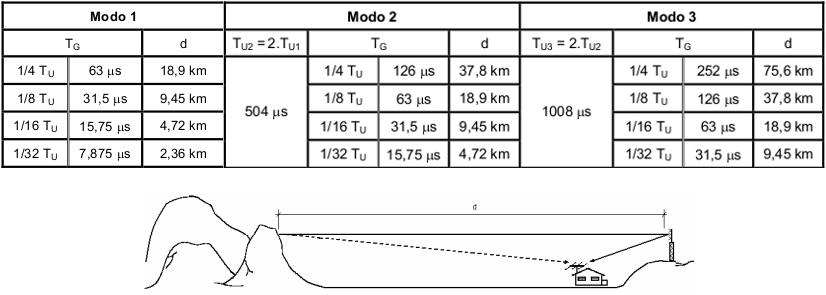
\includegraphics[width=1.15 \textwidth,
keepaspectratio]{/home/delivery/Desktop/TVPILatex/Figuras/Fig33.png}
\caption{\emph{Intervalos de guarda y distancias m\'aximas de
reflexi\'on paara los Modos 1,2, y 3 (Pisciotta N. O; 2010 {``}Sistema
ISDB-Tb (Serie de Materiales de Investigaci\'on - Primera parte - Pag
22)}}
\end{figure}

\begin{center}
\color{white}{.}
\end{center}
\newpage

Realizamos el estudio para el \textbf{\emph{Modo 1}} ya que el mismo
presenta la mayor separaci\'on entre portadoras en el espectro OFDM,
otorgando mayor robustes. Para nuestra implementaci\'on la robustes de
la se\~nal es un requisito indispensable debido a que deseamos Tx un
servicio de TV-Movil One-Seg.
\\
 
Lamentablemente, luego de realizar todas las posibles configuraciones
la distancia de cobertura d $\ge$ 18,1 Km por lo que no fue viable
continuar con el desarrollo para tal implementaci\'on.
Claramente un \textbf{\emph{Modo 3}} permitir\'ia lograr la
transmisi\'on de la multiprogramación planteada con tasas de Tx (C
Mbps) m\'as altas. Sin embargo, correr\'ian riesgo los Rx-M\'oviles al
demodular el Segmento central de la Tx. Recordemos que las portadoras
estar\'an espaciadas con un intervalo m\'inimo aprox. 900Hz. Planteando
un desfasaje de 100Hz por efecto Dopler, el mismo representar\'ia un
10\% de distorci\'on. Por lo que podr\'ia existir Intermodulaci\'on, la
cual afectar\'ia directa y negativamente el servicio.
\\

Es por todo lo anterior que decidimos optar por el \textbf{\emph{Modo
2}} y teniendo en cuenta las principales variables de configuraci\'on
expuestas a continuac\'on es que se desarrolla el Sist. ISDB-Tb:
 

\begin{figure}[h!] 
\centering
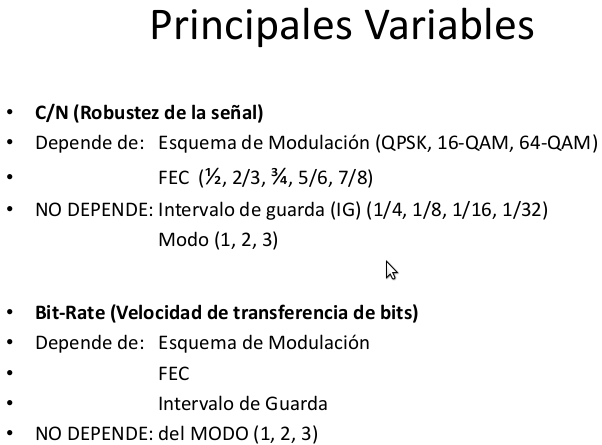
\includegraphics[width=.7 \textwidth,
keepaspectratio]{/home/delivery/Desktop/TVPILatex/Figuras/Fig31.png}
\caption{\emph{Principales Variables para el Dise\~no ISDB-Tb
(Diapositivas tvpi-parte-7-2010 - pag56, Ing. Liendo C.)}}
\end{figure}

\begin{figure}[h!] 
\centering
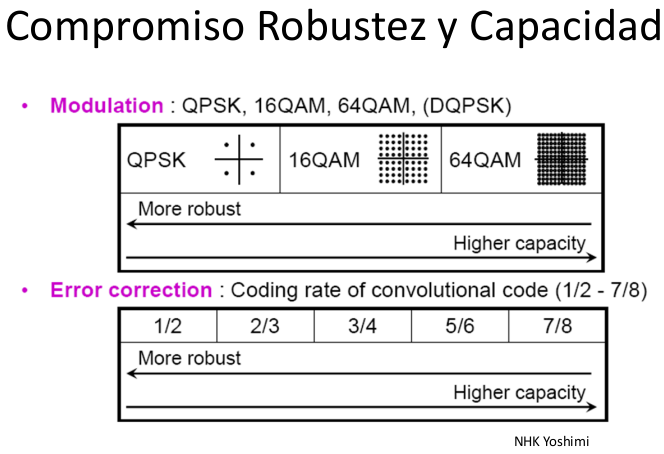
\includegraphics[width=.7 \textwidth,
keepaspectratio]{/home/delivery/Desktop/TVPILatex/Figuras/Fig32.png}
\caption{\emph{Factores que afectan el compromiso Robustez/Capacidad
ISDB-Tb (Diapositivas tvpi-parte-7-2010 - pag58, Ing. Liendo C.)}}
\end{figure}

\newpage
\begin{center}
\color{white}{.}
\end{center}
\newpage

Se procede al An\'alisis del Sistema, haciendo referencia a los
resultados presentados en \textbf{\emph{Subsecci\'on 1.2}}:

\begin{itemize}
\item Par\'ametros comunes a las 3 Capas Jer\'arquicas:
  \begin{itemize}
    \item Modo 2 
    \item Relaci\'on T\textsubscript{G} = \textbf{$\Lambda$ 1/8}
(Haciendo referencia a la \textbf{\emph{Figura23}}      claramente se
cubre la zona deseada y se gana C = Capacidad \'util).
  \end{itemize}
\item Par\'ametros varialbes por Capa Jer\'arquica (A/B/C):
    \begin{itemize}
     \item \textbf{\emph{Capa A:}}
	\subitem $\Rightarrow$ Ki = 2/3
	\subitem $\Rightarrow$ Modul=QPSK(2bist)
	\subitem $\Rightarrow$ Segs = 1
	\subitem $\Rightarrow$ L\textsubscript{D} = 192
	\subitem $\Rightarrow$ T\textsubscript{U} ($\mu$ seg) = 504
	\subitem $\Rightarrow$ T\textsubscript{G} ($\mu$ seg) = 63
	\subitem $\Rightarrow$ T\textsubscript{S} ($\mu$ seg) = 567
	\subitem $\Rightarrow$ Prog = LD (One-Seg)
	\subitem $\Rightarrow$ R (Mbps) = 0,411
    \item \textbf{\emph{Capa B:}}
	\subitem $\Rightarrow$ Ki = 7/8
	\subitem $\Rightarrow$ Modul= 64-QAM(6bist)
	\subitem $\Rightarrow$ Segs = 4
	\subitem $\Rightarrow$ L\textsubscript{D} = 192
	\subitem $\Rightarrow$ T\textsubscript{U} ($\mu$ seg) = 504
	\subitem $\Rightarrow$ T\textsubscript{G} ($\mu$ seg) = 63
	\subitem $\Rightarrow$ T\textsubscript{S} ($\mu$ seg) = 567
	\subitem $\Rightarrow$ Prog = SD + SD + Datos
	\subitem $\Rightarrow$ R (Mbps) = 3 + 3 + 0,5 = 6,5
    \item \textbf{\emph{Capa C:}}
	\subitem $\Rightarrow$ Ki = 7/8
	\subitem $\Rightarrow$ Modul= 64(6bist)
	\subitem $\Rightarrow$ Segs = 8
	\subitem $\Rightarrow$ L\textsubscript{D} = 192
	\subitem $\Rightarrow$ T\textsubscript{U} ($\mu$ seg) = 504
	\subitem $\Rightarrow$ T\textsubscript{G} ($\mu$ seg) = 63
	\subitem $\Rightarrow$ T\textsubscript{S} ($\mu$ seg) = 567
	\subitem $\Rightarrow$ Prog = HD
	\subitem $\Rightarrow$ R (Mbps) = 13
  \end{itemize}
\end{itemize}

Las f\'ormulas impementadas en la Calculadora ISDB-Tb utilizadas fueron:

\begin{flushleft}
\begin{eqnarray}
%Tasa \'util por capa & \ \ \ \ \ \ \ \ \ \ \ \ \ \  \
R_{CAPAx} = & k_0 . k_i . \frac{b_p \times N_{seg} \times
L_D}{T_s} \\
%Cantidad de TSPs \times Capa & \ 
N_{CAPAx} = & \frac{k_i \times b_p \times L_D \times N_seg }{8} \\
%TSP_{s \ no \ nulos} & \ 
TSP_{no \ nulos} = & N_{CAPA A} + N_{CAPA
B} + N_{CAPA C} \\
TSP_{nulos} = & TSP_{s \ Modo2} - TSP_{no \ nulos}  \\
R_{CAPAx \ TOTALES } = & \ \frac{N_{CAPA \ x} \times 204 \times
8}{204 \times T_s}  
\end{eqnarray}
\end{flushleft}

\subsection{Instalaci\'on de los Encoders/Mux/Re-Multiplexor en Canal 10
(Tx BTS)}

En el caso de instalar el Re-Mux estar\'iamos modificando parcialmente
la propuesta de las \textbf{\emph{Subsecciones 1.2 y 1.3}}.
Consecuentemente deber\'iamos incrementar el BW del radio enlace a la
planta Tx. de cerro Mogote. Aunque, recordando la capacidad del Re-Mux
de transmitir solo los $TSP_{no \ nulos}$ mediante un flujo $BTS_c$. De
esta manera se podr\'ia seleccionar el radio \textbf\emph{{Motorola PTP
300 - 25 Mbps}} para compensar la modificaci\'on en la capacidad de
transporte de datos.
Como puntos positivos tendr\'iamos la opci\'on de incrementar la
robustez mediante la codificaci\'on Reed-Solom. En 2do lugar el soporte
del mismo ser\'ia m\'as accesible por su disposici\'on en las
instalaciones de Canal 10.

%\footnote{Nota al pie de la página!}%%%%%%%%%%%%%%%%%%%%%%%%%%%%%%%%%%%

\newpage
\section{Visita a los servicios de Radio y Televisi\'on de la UNC
LV80 TV Canal 10)}

Se realiz\'o una visita guiada el d\'ia Jueves 17 de Noviembre a las
instalaciones de Canal 10 de Córdoba. Las explicaciones estuvieron a
cargo del personal técnico del Canal.
\\
\\

\textbf{\emph{\large{Desarrollo:}}}
\\

El alumno obtendrá información de la exposición del personal técnico, y
efectuará las consultas necesarias para completar el cuestionario.
La emisora se encuentra en un proceso de digitalización en las áreas de
producción de programas, operación de transmisión y producción de
noticieros. A futuro digitalizará la transmisión hasta el televidente.
Esto le permitirá al alumno hacer consultas sobre las características de
las últimas tecnologías digitales.


\newpage
\subsection{Diagrama en bloques emisora}

\begin{figure}[h!] 
\centering
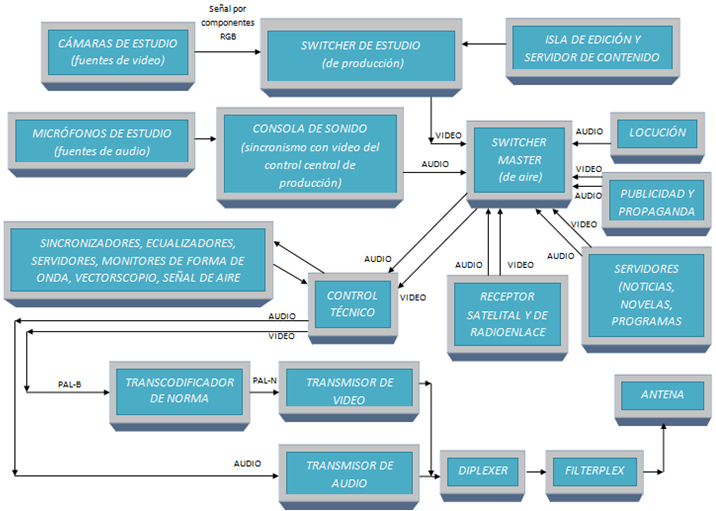
\includegraphics[width=1.15 \textwidth,
keepaspectratio]{/home/delivery/Desktop/TVPILatex/Figuras/Fig23.png}
\caption{\emph{Diagrama en bloques que incluye los dispositivos y
componentes m\'as relevantes de las instalaciones de Canal 10.}}
\end{figure}

\subsection{Partes del Sistema en las que intervienen los conceptos de
Colorimetr\'ia}

Los conceptos adquiridos en colorimetría intervienen en las siguientes
partes:

\begin{itemize}
 \item Estudio: en todo lo relacionado a la calibración de las cámaras,
escenografía (materiales, colores, texturas) e iluminación (temperatura
de color, filtros). 
 \item Consola de luces: al manejar la intensidad de la iluminación con
los drimer.
 \item Control Técnico: donde se controla la ecualización para no
“quemar” la imagen o que quede demasiado “apagada”.
\end{itemize}

\subsection{Partes del Sistema donde interviene directamente el
Monitor de forma de onda y el Vectorscopio)}

El Vectorscopio y el Monitor de Forma de Onda los vimos presentes en
el  Control Técnico tanto para las señales de generación interna como
para las provenientes de otros servicios como direc tv, en versiones
digitales y analógicas, también en la sala donde se ubicaban el
transmisor de tv estaba presente el  Monitor de Forma de Onda para
observar la señal antes de ser transmitida.

Se muestran a continuaci\'on los Monitores de forma de onda (Analogico
y Digital) y Vectorscopio (Integrado al Monitor de onda Digital):

\begin{figure}[h!] 
\centering
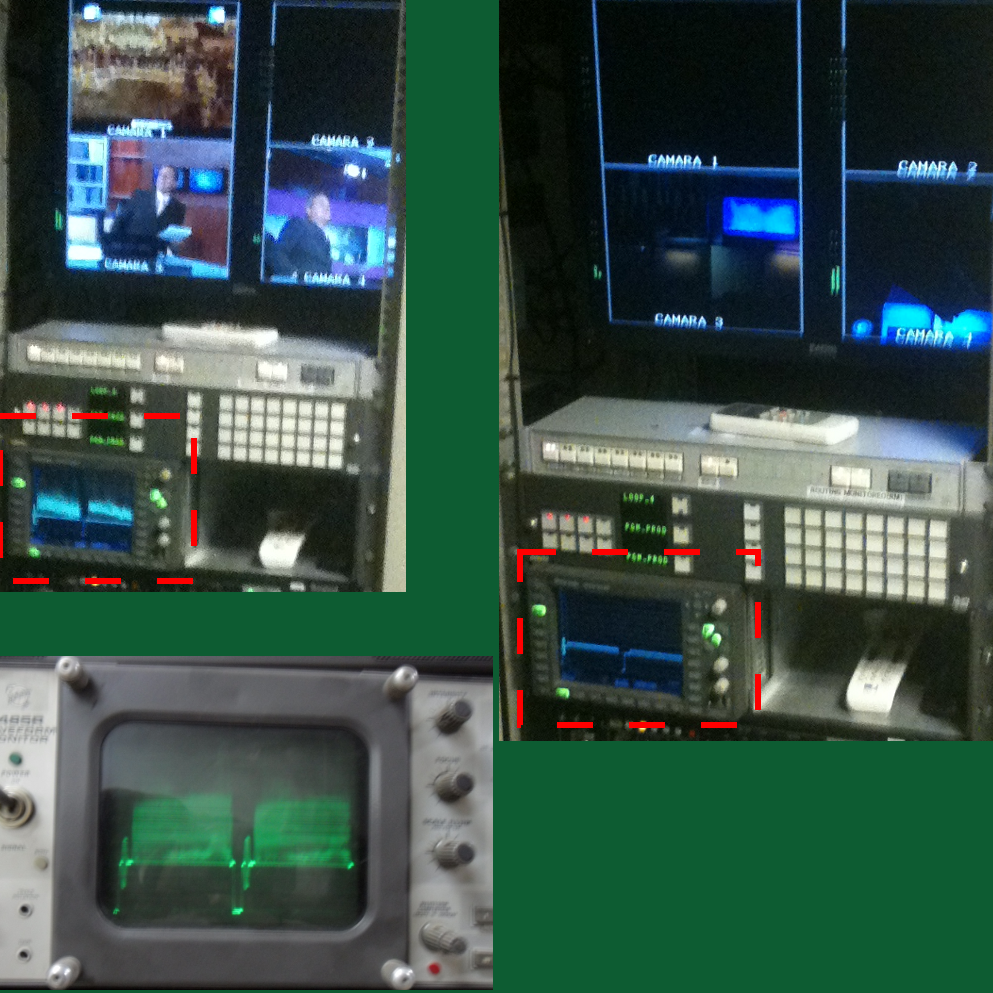
\includegraphics[width=.9 \textwidth,
keepaspectratio]{/home/delivery/Desktop/TVPILatex/Figuras/Fig24.png}
\caption{\emph{Monitores de forma de onda y vectorscopio Canal 10.}}
\end{figure}


\newpage
\subsection{Sistema de ingesta, almacenamiento y
distribución de video y audio}

\begin{figure}[h!] 
\centering
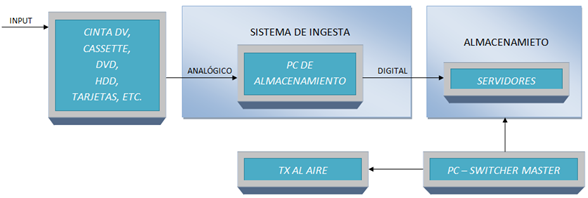
\includegraphics[width=.9 \textwidth,
keepaspectratio]{/home/delivery/Desktop/TVPILatex/Figuras/Fig25.png}
\caption{\emph{Diagrama específico del sistema de ingesta,
almacenamiento y distribución de video y audio utilizando computadoras
en red.}}
\end{figure}

Todo el sistema de ingesta es utilizado por el switcher master y el
control central para la distribución del contenido de la programación
del canal. En el mismo se dispone tanto de audio, video, comerciales,
clips,  donde pueden ser gestionados y se puede hacer un control de los
videoservidores y el equipamiento broadcast, además del control de
realización que le permite a las pc’s de los editores de noticias
digitalizar su contenido, compartirlo con otras estaciones de captura,
etc. Se han dividido las áreas de trabajo a través de servidores, uno de
noticias y otros, por ejemplo, para novelas.
Algunos sistemas de ingesta:

\begin{figure}[h!] 
\centering
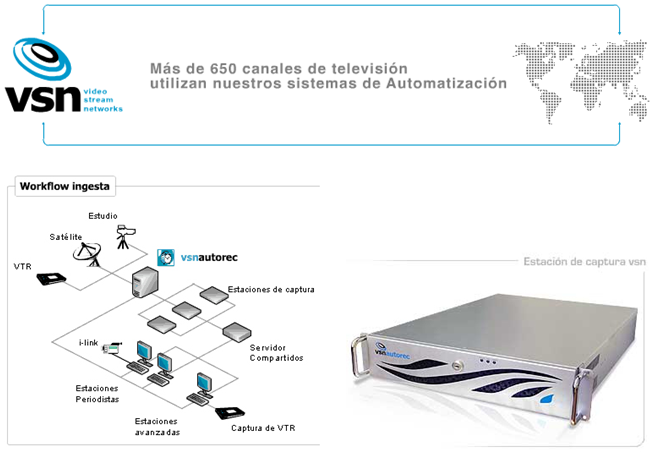
\includegraphics[width=.9 \textwidth,
keepaspectratio]{/home/delivery/Desktop/TVPILatex/Figuras/Fig26.png}
\caption{\emph{Diagrama Sistema de Ingesta VNC.}}
\end{figure}

\newpage
\textbf{Ingesta (vsnautorec)} 
\\

\textbf{\emph{vsnautorec}} es el sistema de ingesta de vtrs y líneas
simultáneas de satélite o estudio, en modo automático o manual. Se
pueden programar capturas periódicas o puntuales de líneas de agencia,
asociadas a una reclist introduciendo la duración el día y la hora
exacta. 
\\

\textbf{\emph{vsnautorec director}} controla el switcher a/v de
contribución y enruta la señal de satélite hacia la estación de captura
disponible en ese momento. Almacena las capturas en los servidores
diarios por categorías y soporta la edición simultánea un minuto después
de empezar a grabar utilizando tecnología Chunking.
\\

\textbf{\emph{vsnautorec capture}} son las estaciones de ingesta
dedicadas, codifican video en formatos DV25, MPEG-2 4:2:0, 4:2:2 a 50
Mbps y Windows Media 9.
\\

\textbf{\emph{vsnautorec terminal}} es la versión remota, que permite a
los PC de los periodistas digitalizar de vtrs compartidos conectados a
la matriz con las estaciones de captura dedicadas. Los usuarios
controlan de forma remota los vtrs sin necesidad de cableado a/v en la
sala de redacción, el sistema gestiona colas de espera en la solicitud
de vtrs y solapamientos con las capturas de las líneas programadas y
manuales.
\\

Todo la ingesta se controla desde el PC del periodista, la visualización
del previo de la captura es en baja resolución por video streaming con
Windows Media 9.
\\

El sistema crea en background una versión en baja resolución de los
materiales capturados para búsquedas y edición, sin ocupar el ancho de
banda de la red, dedicado a la edición en alta resolución. vsnautorec
cubre todas las necesidades de ingesta para noticias y comerciales,
programas para vsnmatic, el playout de control maestro, sin la
intervención de técnicos dedicados.

\begin{figure}[h!] 
\centering
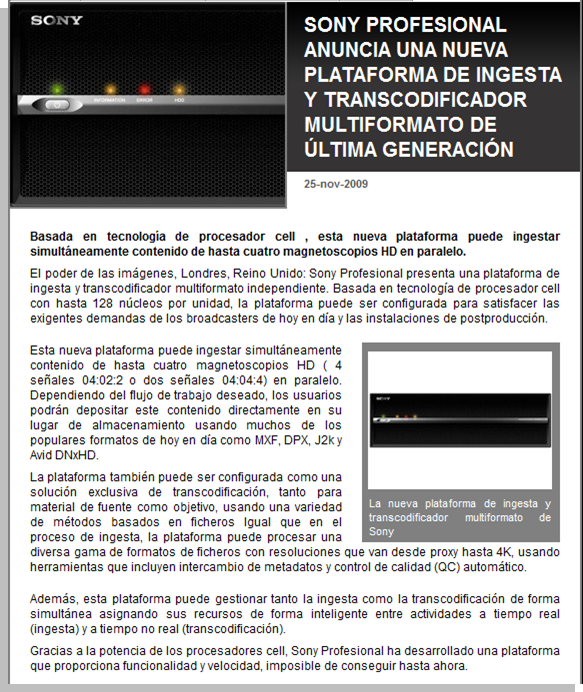
\includegraphics[width=1 \textwidth,
keepaspectratio]{/home/delivery/Desktop/TVPILatex/Figuras/Fig27.png}
\caption{\emph{Plataforma de Ingesta SONY.}}
\end{figure}

\newpage
\subsection{Ecualizadores de Audio y Video}

Los ecualizadores modifican el contenido en frecuencias de las señales
que procesan por medio de filtros que les permiten aumentar o disminuir
un grupo de frecuencias definidas para obtener una respuesta deseada.
Los ecualizadores de video, actúan sobre la fase de las señales, en
lugar de actuar sobre la amplitud como lo hacen los ecualizadores de
audio.

\newpage
\subsection{Funcionamiento del \textbf{\emph{Genlock}}}

\textbf{GENLOCK} \textbf{\emph{(Generator Lock)}}: Este aparato es un
generador de sincronismos y se utiliza en equipos de video avanzados que
deben estar sincronizados para poder procesar o conmutar los videos.
Funciona con una técnica común en video donde una referencia de video
específica sirve para sincronizar 2 o mas fuente de vídeo. Es decir, se
ponen en fase la subportadora y los sincronismos verticales y
horizontales con respecto al patrón de referencia, principalmente para
que al editar las señales estas coincidan y no haya saltos (coincidentes
en sincronismos vertical y horizontal). Por lo tanto cuando dos señales
coinciden se denominan: "genlocked" o sincronizadas.

\subsection{Switcher Master}

La función del Switch Master es la de hacer la selección de audio y
video que se le provee de diferentes fuentes (producción interna,
proveniente de una señal exterior vía satélite o radioenlace, servidor
de contenidos, publicidad, etc.)  y ponerlas al aire respetando una
programación previamente establecida. El Switch Master de canal 10 es
analógico y próximamente reemplazado por uno digital pero no está
preparado para trabajar en HDTV sino solo en SD.

\subsection{Norma analógica empleada por Canal 10 (Estudios -
Producci\'on - Tx)}

La norma que emplea Canal 10 en Estudios y Producción es PAL-B ya que no
se fabrican equipos de normal PAL-N para estas instancias, si no que, se
procesa todo en PAL-B y luego antes de transmitir se hace una
transcodificacion de PAL-B a PAL-N.

\subsection{Se\~nal Compuesta de Video Color en BB y su
Transcodificaci\'on}

La señal de vídeo estándar (también conocida como Señal de Vídeo
Compuesta en Banda Base, o CVBS), llega hasta el transcodificador de
norma que está en la planta transmisora, contiene información de la
sincronización de la pantalla y del blanco y negro junto con la
información de color, todo en una señal.
El bloque transcodificador de normas, pasa la señal de video de Pal-B a
Pal-N antes de multiplexarla con la señal de audio, una ves juntas pasan
por el bloque del Diplexer (éste permite combnar la señal de la antena
local o compañía de cable con la señal de satélite), luego por el
filteplexer (filtro para la señal) y finalmente es transmitida a través
de la antena.

\newpage
\subsection{Cableados SDI}

\textbf{La interfaz digital serial}, \textbf{\emph{(Serial digital
interface (SDI))}} se refiere a la familia de interfaces estandarizadas
para SMPTE. Estos estándares son usados para la transmisión de señales
de video digital no comprimido y no encriptado (opcionalmente incluyendo
audio embebido y/o Código de Tiempo -Time Code-) dentro de las
instalaciones de la televisora; pueden ser también usados para datos
paquetizados. Son diseñados para operaciones sobre cortas distancias
(menores que 300 m. con cable coaxil); debido a sus bit rates altos, son
inadecuados para transmisiones a largas distancias. SDI y HD-SDI están
en la actualidad solo  disponibles en equipamientos de video
profesional; ya que hay varios acuerdos de licenciamiento en que
prohíben su uso en equipos de consumo. Hay varios “mod kits” para
reproductores de DVD y otros dispositivos, que permiten al usuario
añadir una interfaz digital en serie a éstos dispositivos.

\begin{figure}[h!] 
\centering
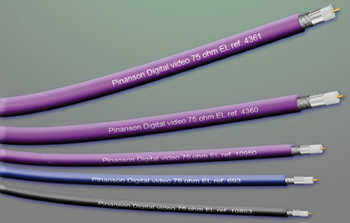
\includegraphics[width=.8 \textwidth,
keepaspectratio]{/home/delivery/Desktop/TVPILatex/Figuras/Fig28.png}
\caption{\emph{Plataforma de Ingesta SONY.}}
\end{figure}

\textbf{Cables de video digital SDI/HDTV, aplicaciones:}
\\

Estudios de Televisión y unidades móviles.
Cables coaxiales de video para aplicaciones digitales y analógicas
críticas.
Soporta transmisión de datos seriadas (SDI) y formato de televisión de
Alta definición (HDTV)


\begin{figure}[h!] 
\centering
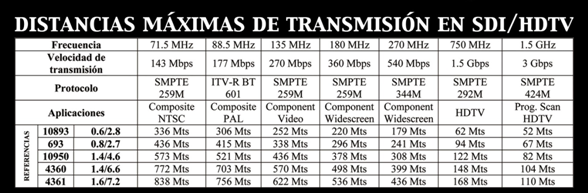
\includegraphics[width=1.1 \textwidth,
keepaspectratio]{/home/delivery/Desktop/TVPILatex/Figuras/Fig29.png}
\caption{\emph{Plataforma de Ingesta SONY.}}
\end{figure}

\newpage
En el estudio de canal 10 según lo comentado se utiliza SDI hasta el
switch de producción.

\subsection{\textbf{\emph{CBA24N}}: Tecnolog\'ia y forma de Tx}
En base a lo expuesto por el personal t\'ecnico durante la visita a
Canal 10 podemos sintetizar la tecnolog\'ia implementada de CBA24N como
sigue:

\textbf{CBA24 Noticias}
\\

\begin{itemize}
\item Estudio compartido (CBA24N \ / \ Canal 10).
\item Utilizaci\'on integra de interfazes SDI reemplazando las antiguas:
  \subitem Camaras Digitales (SDI). En Standar SD. En un futuro existe
la posibilidad de implementar programaci\'on en HD por lo que se
instalar\'a un Fibra \'Optica en lugar del Radio Enlace Analog con la
planta Tx. del cerro Mogote.
  \subitem Master Switcher SDI (Rx se\~nal camaras) en conjunto con
Soft administran la programaci\'on que ser\'a emitida al aire. Los
programas que no son en vivo, ser\'an almacenados en un Servidor
intermedio para ser reproducidos en el momento deseado.
\item Consola de sonido profesional Anal\'ogica (CBA24N \ / \ Canal 10)
\item 3 Servidores: 
  \subitem Noticas
  \subitem Producci\'on
  \subitem Comerciales 
\item 3 Generadores de Sincronismo patr\'on (2 Analog. + 1 Dig)
evitando el desfasaje de las se\~nales con respecto a un pulso de
referencia. 
\end{itemize}

Nota: La Tx. de CBA24 es en SDI, mientas que la de Canal 10 se trata de
SCVC. En los Switchers Masters ingresan A/V siendo transmitidos de
forma embebida en un mismo paquete. 
 
\newpage
\section{Referencias}

\textbf{\emph{1.}} Notas Visita Canal 10 17/11/2011.
\\

\textbf{\emph{2.}} Pisciotta N. O; 2010 {``}Sistema ISDB-Tb
(Serie de Materiales de Investigaci\'on - Primera parte)''.
\\

\textbf{\emph{3.}} Liendo C.; 2010 {``}tvpi-parte-7-2010 (Filminas
ISDB-Tb)''.


\end{document}


\begin{comment}

\begin{figure}[!htb] 
\centering
\includegraphics[width=.8\textwidth,
keepaspectratio]{/home/delivery/Desktop/RCIILatex/Figuras/Fig10.png}
\caption{\emph{Patch rectangular con la distribuci\'{o}n de densidad de
corriente magn\'{e}tica en las ranuras} para el modo
\textbf{TM}\textbf{\textsubscript{100}}.\emph{\textbf{b)}
distribuci\'{o}n de corriente en las ranuras no radiantes.}} 
\end{figure}

\begin{table}[htb]
\centering
\caption{\emph{Algunos campos de aplicaci\'{o}n donde se utilizan
antenas patch.}}
\\[.1cm]%%%%%%%%%%%%%%%%%%%%%%%%%%%%%%%%%%%%%%%%%%%%%%%%%%%%%%%%%%%%%%
%
% Table begins
%
\begin{tabular}[htb]{|l|p{7.4cm}|}
\hline 
\textbf{Campo de aplicaci\'on} & \textbf{Tipo de sistema}  
                                                  \\
\hline
Naves espaciales               & Radar, comunicaciones, navegación 
altímetros y sistemas de aterrizaje       
                                                   \\
\hline                                            
Misiles                        & Radar, telemetr\'ia 
						   \\              
\hline
Sat\'elites                    & Comunicaciones, TV de difusióndirecta,
                                                   \\                
			       & radares de censado remoto y
radiómetros                                                    
						   \\
\hline
Aviones                        & Radar, comunicaciones, navegación 
                                                   \\
\hline                                            
Veh\'iculos                    & Teléfonos móviles satelitales, radio
móvil                                              \\
\hline
Otros                          & Sistemas biomédicos, alarmas contra
intrusos                                           \\
\hline
\end{tabular}
\end{table}

\begin{itemize}
\item \textbf{Antenas de patch microstrip } 
\item Dipolos microstrip
\item Antenas de ranura impresa 
\item Antenas microstrip de onda viajera
\end{itemize}

\begin{center}
\begin{math}
\varepsilon_{reff} = \frac{\varepsilon_r+1}{2} +
[\frac{(\varepsilon_r-1)}{2} *(1 + 12 \times \frac{h}{W})]^{1/2} \ ;  \
con \ W/h > 1
\end{math}
\end{center}

\begin{center}
\begin{eqnarray}
J_s= & \ n \times H_a \\
M_s= & \-n \times E_a
\end{eqnarray}
\end{center}

\begin{center}
\begin{math}
E_a= \ z \times E_0 
\end{math}
\end{center}

\begin{center}
\begin{math}
E_a= \ -E_0 \times \sin(\pi L)  
\end{math}
\end{center}

 delivery@delivery-pc:~/Desktop/LaTex $ ls -l
total 1136
-rw-r--r-- 1 delivery delivery 1032355 2011-09-03 09:51 curso_LaTeX.pdf
-rw-r--r-- 1 delivery delivery    2567 2011-09-03 11:06 Latex_course_notes
-rw-r--r-- 1 delivery delivery     396 2011-09-03 12:06 PrimerArchivo.aux
-rw-r--r-- 1 delivery delivery     864 2011-09-03 12:05 PrimerArchivo.dvi
-rw-r--r-- 1 delivery delivery    5609 2011-09-03 12:06 PrimerArchivo.log
-rw-r--r-- 1 delivery delivery   25439 2011-09-03 12:06 PrimerArchivo.pdf
-rw-r--r-- 1 delivery delivery     656 2011-09-03 12:05 PrimerArchivo.tex
-rw-r--r-- 1 delivery delivery     657 2011-09-03 12:05 PrimerArchivo.tex~
delivery@delivery-pc:~/Desktop/LaTex $ evince PrimerArchivo.pdf

Para compilar desde consola:
delivery@delivery-pc:~/Desktop/LaTex $ latex PrimerArchivo.tex && dvipdf
PrimerArchivo.dvi 

con ``?'' tratará de compilar
con ``quit`` termina la compilación

\end{comment}

